\documentclass[11pt]{article}
\usepackage[margin=1in]{geometry}
\usepackage{amsmath,amssymb}
\usepackage{graphicx}
\usepackage{booktabs}
\usepackage{enumitem}
\usepackage[colorlinks=true,linkcolor=black,urlcolor=blue]{hyperref}
\usepackage{xcolor}
\usepackage{float}
\usepackage{caption}
\usepackage{pdflscape}
\captionsetup{font=small,labelfont=bf}

\newcommand{\net}{\mathrm{net}}
\newcommand{\bw}{\mathbf{w}}
\newcommand{\bp}{\mathbf{p}}
\newcommand{\bx}{\mathbf{x}}

\title{\vspace{-1.2cm}\textbf{Homework 1}}
\author{CS 4033/5033, Machine Learning Fundamentals, Fall 2026}
\date{Ridwan Hoque}

\begin{document}
\maketitle
\vspace{-0.8cm}

\noindent\rule{\textwidth}{0.4pt}

\section*{Part 1: AN Representation}

\subsection*{Preliminary: why we augment the input vector}

In a standard neural network layer, the math that we need to perform in order to
calculate the output $y$ requires two separate operations: a matrix multiplication
and a vector addition.
\[
y \;=\; W\bx + b ,
\]
where $\bx$ is the input vector (for example, the features or the data points),
$W$ is the weight matrix, and $b$ is the bias vector, which shifts the activation
function.

In code and in hardware such as GPUs, having to multiply and then add separately
slows down processing, because we have to perform two distinct memory operations
rather than one.

\paragraph{The solution: the augmented vector trick.}
By augmenting the input vector with a constant $1$, we are able to fuse the weight
and the bias together into a single, highly optimized matrix multiplication step.

\medskip
\noindent\textbf{Step 1: augment the input vector.}
We need to take the original input vector $\bx$ and append a $1$ at the very bottom:
\[
\bx_{\text{aug}} \;=\;
\begin{bmatrix} x_1 \\ x_2 \\ \mathbf{1} \end{bmatrix} .
\]

\noindent\textbf{Step 2: augment the weight matrix.}
We need to take the original weight matrix $W$ and append the bias vector $b$ as an
extra column at the end:
\[
W_{\text{aug}} \;=\;
\begin{bmatrix}
w_{11} & w_{12} & \mathbf{b_1} \\
w_{21} & w_{22} & \mathbf{b_2}
\end{bmatrix} .
\]

\noindent\textbf{The clean result.}
The neural network now only has to perform one single multiplication:
\[
y \;=\; W_{\text{aug}} \cdot \bx_{\text{aug}} .
\]
If we write this out, the math naturally multiplies the weights by the inputs and
automatically adds the bias at the end, because the bias column gets multiplied by
the constant $1$.

This is exactly the convention that the rest of this assignment uses. Throughout, we
have to work with the augmented input $\bp = (1,\,x_1,\,x_2)$ and the augmented weight
vector $\bw = (w_0,\,w_1,\,w_2)$, so that the threshold test reduces to the single
condition $\bw \cdot \bp \ge 0$.

\subsection*{1.1\quad Draw the AN}

The artificial neuron has an augmented input vector
$\bp = (x_0, x_1, x_2) = (1, x_1, x_2)$ and a weight vector
$\bw = (w_0, w_1, w_2) = (0.5,\; 1.0,\; -0.3)$. The summation unit computes

\[
\net \;=\; \bw \cdot \bp \;=\; w_0 x_0 + w_1 x_1 + w_2 x_2 \;=\; 0.5 + 1.0\,x_1 - 0.3\,x_2 ,
\]

and the step activation produces the output
\[
a \;=\; f(\net) \;=\;
\begin{cases}
1, & \net \ge 0,\\[2pt]
0, & \net < 0 .
\end{cases}
\]

\begin{figure}[H]
\centering
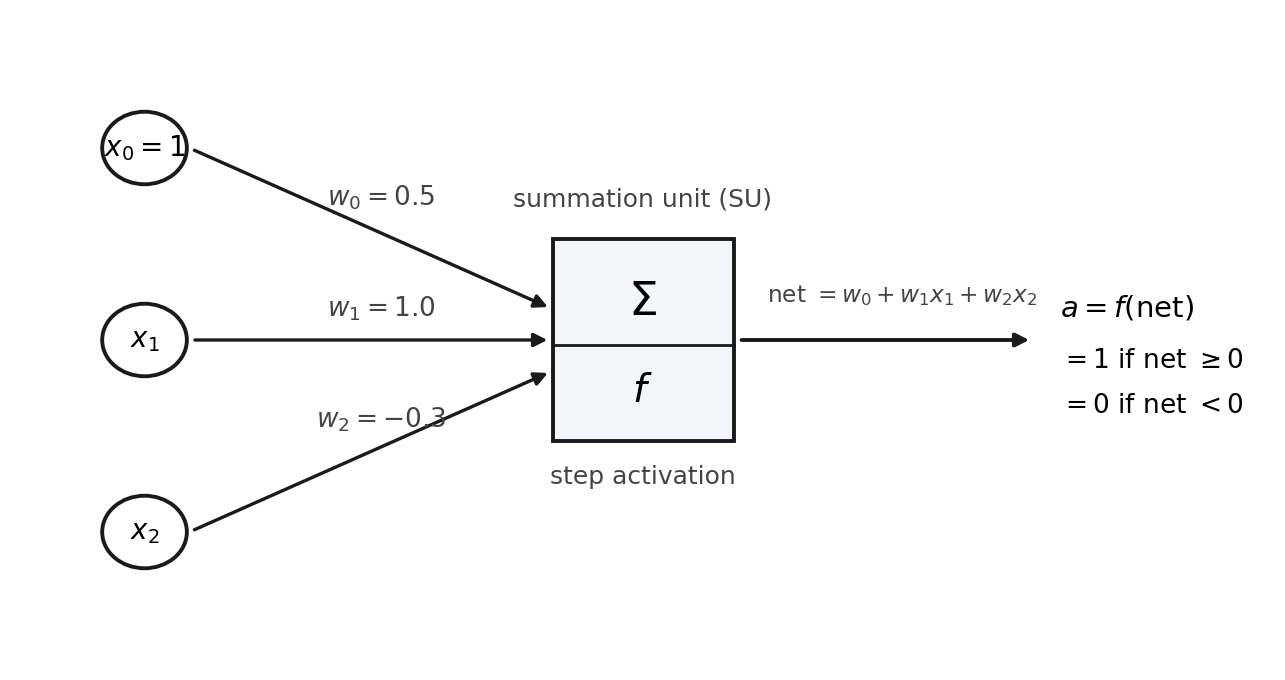
\includegraphics[width=0.92\textwidth]{figures/fig1_an.png}
\caption{The artificial neuron. The constant input $x_0 = 1$ carries the bias weight $w_0$,
so the threshold is absorbed into the weight vector and the test becomes simply
$\bw\cdot\bp \ge 0$.}
\end{figure}

\subsection*{1.2\quad Decision boundary}

The boundary is the locus where the neuron switches its output; that is, where $\net = 0$:
\[
0.5 + x_1 - 0.3\,x_2 = 0
\qquad\Longleftrightarrow\qquad
x_2 = \frac{0.5 + x_1}{0.3} = \frac{5 + 10x_1}{3}.
\]

This is a straight line with slope $10/3 \approx 3.33$, with $x_2$-intercept
$5/3 \approx 1.67$ (at $x_1 = 0$) and $x_1$-intercept $-0.5$ (at $x_2 = 0$).

\paragraph{Which side is the ``front''?}
The vector of non-bias weights $(w_1, w_2) = (1.0,\,-0.3)$ is normal to the line, and it
points into the half-plane where $\net$ increases; that is, toward Class~1. Moving in the
direction $(1.0, -0.3)$ means moving right and slightly down, so the Class~1 (``front'')
side is the lower-right half-plane. As a check, we need to evaluate the origin $(0,0)$,
which gives $\net = 0.5 \ge 0$, so the origin lies on the Class~1 side.

\begin{figure}[H]
\centering
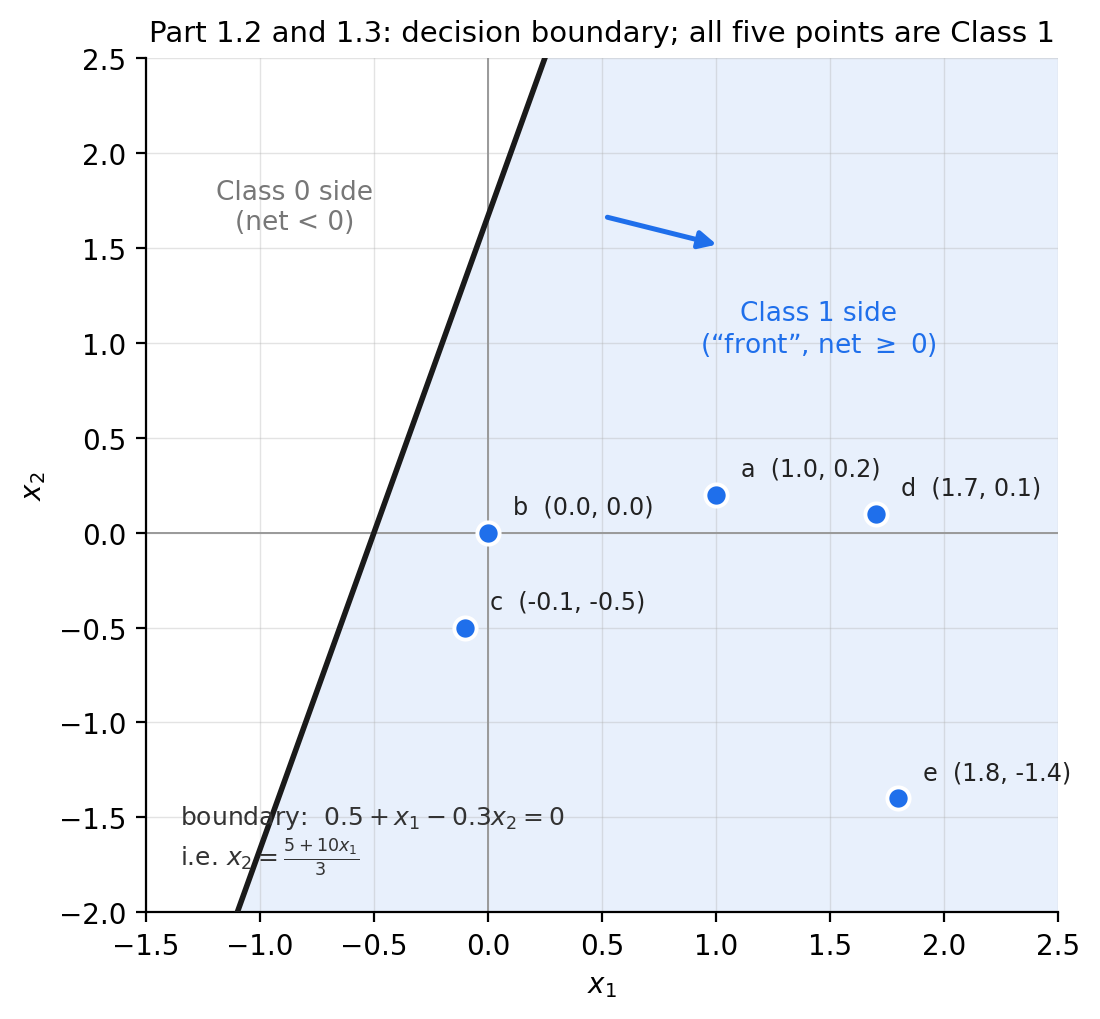
\includegraphics[width=0.62\textwidth]{figures/fig2_boundary.png}
\caption{The decision boundary $0.5 + x_1 - 0.3x_2 = 0$. The shaded lower-right half-plane
is the ``front'' (Class 1, $\net \ge 0$); the arrow is the weight normal
$(w_1,w_2) = (1.0,-0.3)$. The five points of question 1.3 are plotted, and all five of them
fall on the Class~1 side.}
\end{figure}

\subsection*{1.3\quad Add and label the five points}

\begin{table}[H]
\centering
\begin{tabular}{clcc}
\toprule
& Point $(x_1,x_2)$ & $\net = 0.5 + x_1 - 0.3x_2$ & Class $a=f(\net)$ \\
\midrule
(a) & $(1.0,\;0.2)$    & $0.5 + 1.0 - 0.06 = 1.44$   & \textbf{1} \\
(b) & $(0.0,\;0.0)$    & $0.5 + 0.0 - 0.00 = 0.50$   & \textbf{1} \\
(c) & $(-0.1,\;-0.5)$  & $0.5 - 0.1 + 0.15 = 0.55$   & \textbf{1} \\
(d) & $(1.7,\;0.1)$    & $0.5 + 1.7 - 0.03 = 2.17$   & \textbf{1} \\
(e) & $(1.8,\;-1.4)$   & $0.5 + 1.8 + 0.42 = 2.72$   & \textbf{1} \\
\bottomrule
\end{tabular}
\caption{Every $\net$ value is non-negative, so this AN assigns \emph{all five} points to
Class~1. The points are plotted in Figure 2.}
\end{table}

\subsection*{1.4\quad A new point that forces a misclassification}

\paragraph{The new data item.} We have to add the labeled point
\[
\boxed{\;(0.9,\;-0.7)\ \text{with label Class } 0.\;}
\]

\paragraph{Why no weights can work.} All five of the original points are Class~1, and the
new point is the \emph{midpoint} of two of them:
\[
(0.9,\,-0.7) \;=\; \tfrac{1}{2}\big[(0.0,\,0.0) + (1.8,\,-1.4)\big] \;=\; \tfrac{1}{2}\,(b + e).
\]

Now we need to consider \emph{any} weight vector $\bw = (w_0,w_1,w_2)$ whatsoever. Because
$\net(\bp) = \bw\cdot\bp$ is an affine function of the point, and because the augmented
coordinate $x_0 = 1$ is the same for all three points, the value of $\net$ at the midpoint
is the average of the two end values:
\[
\net\!\left(\tfrac{b+e}{2}\right) \;=\; \tfrac{1}{2}\Big[\net(b) + \net(e)\Big].
\]

Suppose such a $\bw$ classified points $b$ and $e$ correctly. Both of them are Class~1, so
$\net(b) \ge 0$ and $\net(e) \ge 0$. Then
\[
\net\!\left(\tfrac{b+e}{2}\right) \;=\; \tfrac{1}{2}\big[\underbrace{\net(b)}_{\ge 0} + \underbrace{\net(e)}_{\ge 0}\big] \;\ge\; 0 ,
\]
so the AN outputs $a = 1$ at $(0.9,-0.7)$, but that point is labeled Class~0. This is a
contradiction. Hence, for every possible $\bw$, at least one of $\{b,\;e,\;(0.9,-0.7)\}$
has to be misclassified.

\paragraph{The general principle.} A single AN can only realize a \emph{linear} separator,
and a linear separator exists if and only if the convex hulls of the two classes do not
intersect. Any linear half-plane that encloses all of the surrounding Class~1 vertices must
also enclose all of the interior points. Assigning an interior point to Class~0 therefore
creates a data set that is not linearly separable, in the same way that the XOR problem is
not linearly separable, and this makes it impossible for any set of weights
$(w_0, w_1, w_2)$ to classify all of the points correctly. The new point lies strictly
inside the convex hull of the Class~1 points, in fact on the chord joining $b$ and $e$, so
the two hulls overlap.

\begin{figure}[H]
\centering
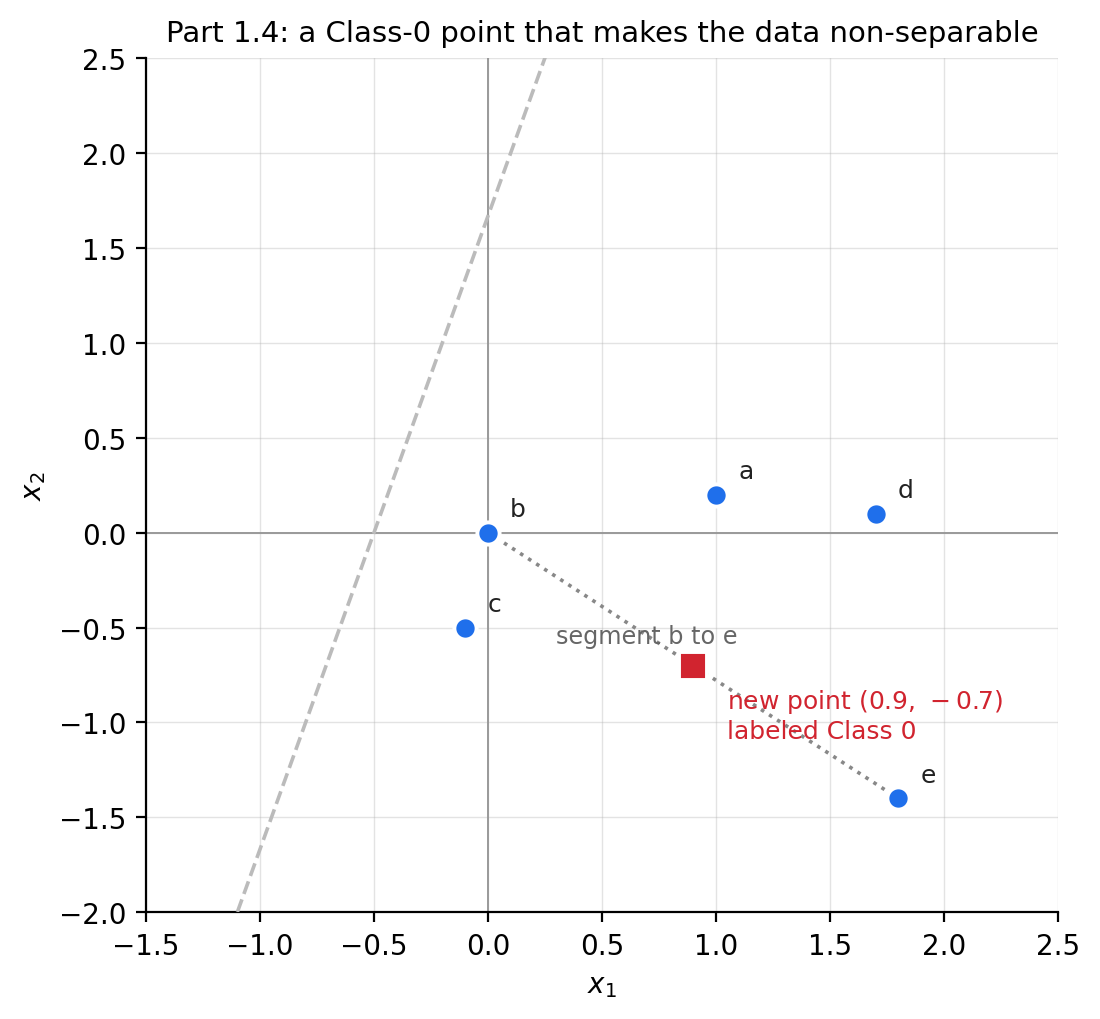
\includegraphics[width=0.60\textwidth]{figures/fig3_nonsep.png}
\caption{The Class-0 point $(0.9,-0.7)$ sits on the segment joining the Class-1 points
$b=(0,0)$ and $e=(1.8,-1.4)$. Any line putting $b$ and $e$ on its positive side must also
put their midpoint there, so no single AN is able to classify all six points correctly.}
\end{figure}

\subsection*{1.5\quad Changing $f$ to output $\{1,-1\}$}

\paragraph{What changes.} \emph{Nothing about the decision boundary.} It remains the same
line $0.5 + x_1 - 0.3x_2 = 0$, with the same slope, the same intercepts, and the same
``front'' side. The only change is the numeric label attached to the negative half-plane:
points that used to produce output $0$ now produce output $-1$.

\paragraph{Why.} The decision boundary is determined entirely by \emph{where the activation
function switches}, and not by the values that it switches between. Both step functions
switch at exactly the same argument, $\net = 0$:
\[
f_{\text{old}}(\net) =
\begin{cases}1, & \net \ge 0\\ 0, & \net < 0\end{cases}
\qquad
f_{\text{new}}(\net) =
\begin{cases}1, & \net \ge 0\\ -1, & \net < 0\end{cases}
\]
Since the geometry of the boundary comes from solving $\net = 0$, an equation that involves
only $\bw$ and $\bp$ and not $f$, and since $f$ is a monotone function of $\net$ in both
cases with its discontinuity at the same place, the partition of the input plane into two
half-planes is identical. Only the \emph{encoding} of the negative class changes, from $0$
to $-1$.

This does matter elsewhere. A $\{-1,1\}$ encoding makes the quantity $t - a$ in a learning
rule equal to $\pm 2$ instead of $\pm 1$, which rescales the size of a weight update.
However, it does not move the boundary for a \emph{fixed} weight vector.

\subsection*{1.6\quad Changing $f$ to the logistic sigmoid}

\paragraph{1. The raw score (net).}
Before we apply any activation function, the neuron calculates a single number called
$\net$, which is a weighted sum of the inputs:
\[
\net \;=\; 0.5 + 1.0\,x_1 - 0.3\,x_2 .
\]
We need to think of $\net$ as a score:
\begin{itemize}[leftmargin=1.4em,itemsep=1pt]
\item Positive score ($\net > 0$): points on the Class 1 side.
\item Negative score ($\net < 0$): points on the Class 0 side.
\item Zero score ($\net = 0$): points sitting directly on the dividing line.
\end{itemize}

\paragraph{2. The step function (hard wall).}
With the step function, the neuron makes a harsh, all-or-nothing decision:
\begin{itemize}[leftmargin=1.4em,itemsep=1pt]
\item If $\net \ge 0 \rightarrow$ output $1$ (Class 1).
\item If $\net < 0 \rightarrow$ output $0$ (Class 0).
\end{itemize}
The switch point, where the output jumps from $0$ to $1$, happens exactly at $\net = 0$.

\paragraph{3. The sigmoid function (smooth ramp).}
The sigmoid function replaces that sharp jump with a smooth curve that outputs numbers
between $0$ and $1$:
\[
\text{output} \;=\; \sigma(\net) \;=\; \frac{1}{1 + e^{-\net}} .
\]
To convert the continuous sigmoid outputs into binary classes, standard classification uses
a $0.5$ threshold:
\begin{itemize}[leftmargin=1.4em,itemsep=1pt]
\item If output $\ge 0.5 \rightarrow$ predict Class 1.
\item If output $< 0.5 \rightarrow$ predict Class 0.
\end{itemize}

\paragraph{4. Why the line stays in the exact same spot.}
We need to look at what happens to the sigmoid equation when the input score is zero:
\[
\sigma(0) \;=\; \frac{1}{1 + e^{0}} \;=\; \frac{1}{1+1} \;=\; \mathbf{0.5} .
\]
\begin{itemize}[leftmargin=1.4em,itemsep=1pt]
\item When $\net = 0$, the sigmoid output is exactly $0.5$.
\item When $\net > 0$, the sigmoid output is greater than $0.5$ (Class 1).
\item When $\net < 0$, the sigmoid output is less than $0.5$ (Class 0).
\end{itemize}
Because the classification threshold is $0.5$, we still have to find the dividing line
between Class 1 and Class 0 by solving $\net = 0$. Since the equation
$0.5 + x_1 - 0.3x_2 = 0$ has not changed, the geometric line plotted on the graph remains
identical.

\paragraph{Summary of what changes and what stays the same.}
\begin{itemize}[leftmargin=1.4em,itemsep=1pt]
\item \textbf{Stays the same:} the geometric boundary line on the graph ($\net = 0$).
\item \textbf{Changes:} instead of a sharp cliff at the boundary, the sigmoid creates a
smooth confidence gradient. Points far from the line get outputs close to $1$ or $0$, which
means high confidence, while points right next to the line get outputs close to $0.5$,
which means low confidence and an undecided result.
\end{itemize}

\begin{figure}[H]
\centering
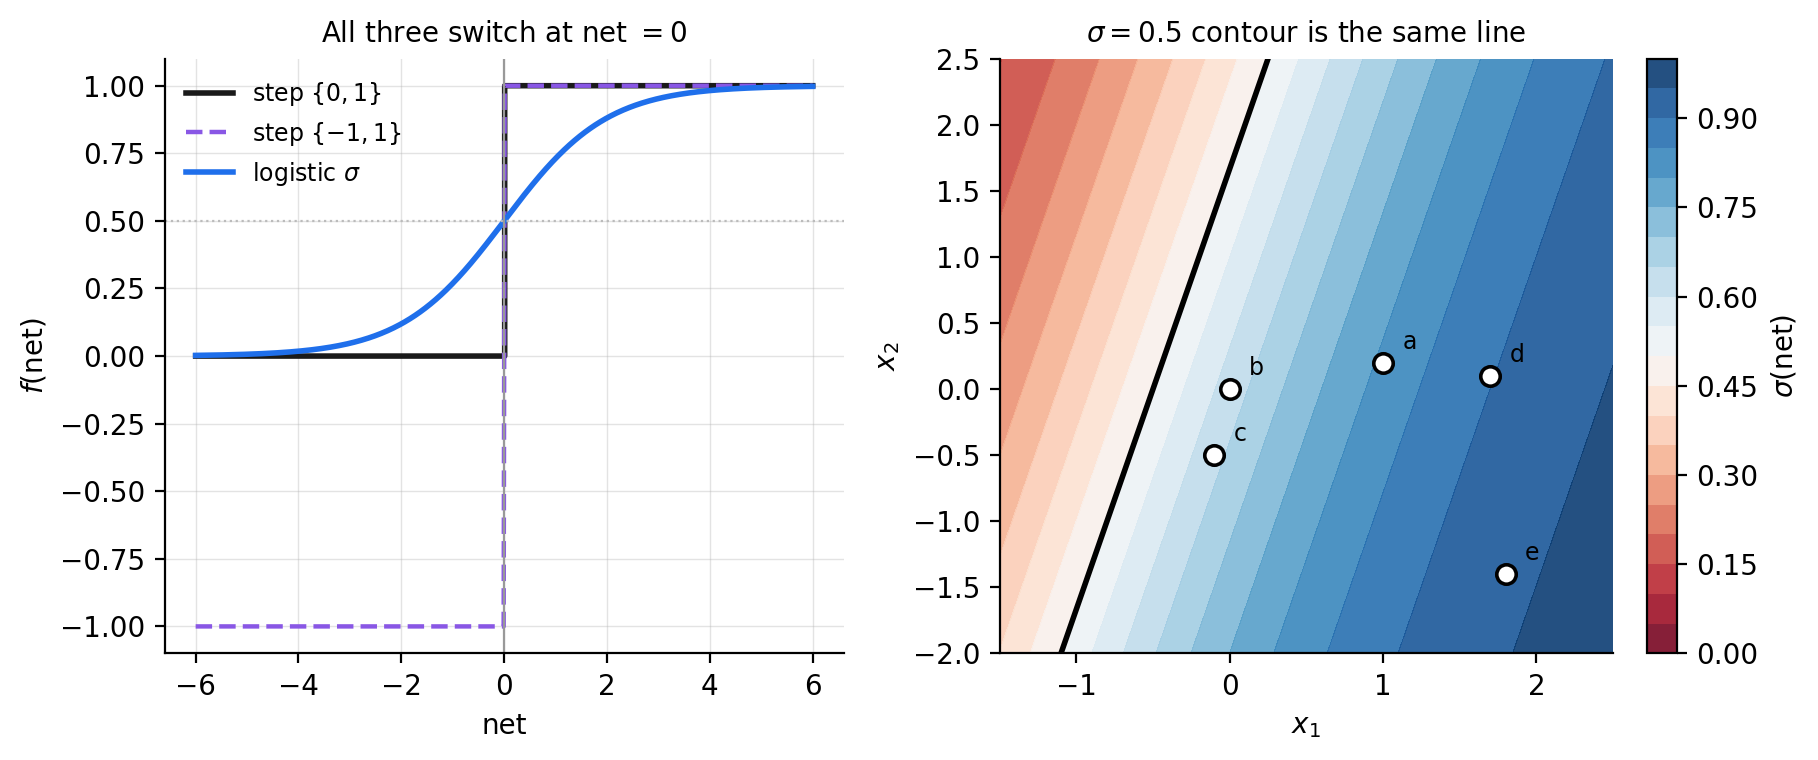
\includegraphics[width=0.95\textwidth]{figures/fig4_sigmoid.png}
\caption{Left: all three activation functions switch at $\net = 0$, so all three give the
same boundary. The step functions differ only in the value assigned to the negative side,
and the sigmoid replaces the jump with a smooth ramp. Right: $\sigma(\net)$ over the input
plane, where the black line is the $\sigma = 0.5$ contour, identical to the boundary of
Figure 2.}
\end{figure}

\subsection*{1.7\quad Classification of the five points under the sigmoid}

\begin{table}[H]
\centering
\begin{tabular}{clccc}
\toprule
& Point & $\net$ & $\sigma(\net) = \frac{1}{1+e^{-\net}}$ & Class (threshold $0.5$) \\
\midrule
(a) & $(1.0,\;0.2)$   & $1.44$ & $0.808$ & 1 \\
(b) & $(0.0,\;0.0)$   & $0.50$ & $0.622$ & 1 \\
(c) & $(-0.1,\;-0.5)$ & $0.55$ & $0.634$ & 1 \\
(d) & $(1.7,\;0.1)$   & $2.17$ & $0.897$ & 1 \\
(e) & $(1.8,\;-1.4)$  & $2.72$ & $0.938$ & 1 \\
\bottomrule
\end{tabular}
\end{table}

\paragraph{Answer.} The classifications \emph{do not change}, and all five points are still
Class~1. What changes is that the AN no longer treats them as equivalent. Under the step
function, every one of these points produced the identical output $1$. Under the sigmoid,
the output grades them by how far they sit from the boundary. Point $e$, which is deepest
inside the Class-1 region, gets $0.938$, while points $b$ and $c$ sit close to the line and
get only about $0.62$ to $0.63$, which means the neuron is barely committed to them. If we
had to use a stricter threshold than $0.5$, for example $0.7$, then $b$ and $c$ would flip
to Class~0, which the step function could never express.

\bigskip
\noindent\rule{\textwidth}{0.4pt}

\section*{Part 2: AN Learning}

Throughout this part, we have to apply the learning rule
\[
\bw_{\text{new}} \;=\; \bw_{\text{old}} + (t - a)\,\bp ,
\]
where $\bp = (1, x_1, x_2)$ is the augmented input, $t \in \{0,1\}$ is the target, and
$a = f(\net)$ is the actual output of the step function of question 1.1. The starting
weights are $\bw = (0.5,\;1.0,\;-0.3)$.

We should note that because $t, a \in \{0,1\}$, the factor $(t - a)$ can only take three
values:
\[
t - a =
\begin{cases}
0 & \text{correct, so we do not need to update,} \\
+1 & \text{predicted 0, should be 1, so we need to add } \bp, \\
-1 & \text{predicted 1, should be 0, so we need to subtract } \bp .
\end{cases}
\]

\subsection*{2.1\quad Weight updates, one pass through the data}

\paragraph{(a) Class 0: $(-0.1,\,-1.0)$, so $\bp = (1,\,-0.1,\,-1.0)$ and $t=0$.}
\begin{align*}
\net &= 0.5 + (1.0)(-0.1) + (-0.3)(-1.0) = 0.5 - 0.1 + 0.3 = 0.70 \;\ge\; 0 \;\Rightarrow\; a = 1 .\\
t - a &= 0 - 1 = -1 \quad \text{(misclassified, so we need to update)}\\
\bw_{\text{new}} &= (0.5,\,1.0,\,-0.3) + (-1)(1,\,-0.1,\,-1.0)
= \mathbf{(-0.5,\;1.1,\;0.7)} .
\end{align*}

\paragraph{(b) Class 0: $(0.2,\,-0.9)$, so $\bp = (1,\,0.2,\,-0.9)$ and $t=0$.}
\begin{align*}
\net &= -0.5 + (1.1)(0.2) + (0.7)(-0.9) = -0.5 + 0.22 - 0.63 = -0.91 \;<\; 0 \;\Rightarrow\; a = 0 .\\
t - a &= 0 - 0 = 0 \quad \text{(correct, so \textbf{no change})}\\
\bw_{\text{new}} &= \mathbf{(-0.5,\;1.1,\;0.7)} .
\end{align*}

\paragraph{(c) Class 1: $(0.6,\,0.8)$, so $\bp = (1,\,0.6,\,0.8)$ and $t=1$.}
\begin{align*}
\net &= -0.5 + (1.1)(0.6) + (0.7)(0.8) = -0.5 + 0.66 + 0.56 = 0.72 \;\ge\; 0 \;\Rightarrow\; a = 1 .\\
t - a &= 1 - 1 = 0 \quad \text{(correct, so \textbf{no change})}\\
\bw_{\text{new}} &= \mathbf{(-0.5,\;1.1,\;0.7)} .
\end{align*}

\paragraph{(d) Class 1: $(0.0,\,0.0)$, so $\bp = (1,\,0.0,\,0.0)$ and $t=1$.}
\begin{align*}
\net &= -0.5 + (1.1)(0) + (0.7)(0) = -0.50 \;<\; 0 \;\Rightarrow\; a = 0 .\\
t - a &= 1 - 0 = +1 \quad \text{(misclassified, so we need to update)}\\
\bw_{\text{new}} &= (-0.5,\,1.1,\,0.7) + (+1)(1,\,0,\,0) = \mathbf{(0.5,\;1.1,\;0.7)} .
\end{align*}

\noindent\textbf{Summary of pass 1.} The following table collects the whole pass.

\begin{table}[H]
\centering
\begin{tabular}{clcccl}
\toprule
Step & $\bp$ & $t$ & $\net$ & $a$ & $\bw$ after the step \\
\midrule
      & (start) & & & & $(0.5,\;1.0,\;-0.3)$ \\
(a) & $(1,-0.1,-1.0)$ & 0 & $+0.70$ & 1 & $(-0.5,\;1.1,\;0.7)$ \quad \emph{updated} \\
(b) & $(1,\;0.2,-0.9)$ & 0 & $-0.91$ & 0 & $(-0.5,\;1.1,\;0.7)$ \quad no change \\
(c) & $(1,\;0.6,\;0.8)$ & 1 & $+0.72$ & 1 & $(-0.5,\;1.1,\;0.7)$ \quad no change \\
(d) & $(1,\;0.0,\;0.0)$ & 1 & $-0.50$ & 0 & $(0.5,\;1.1,\;0.7)$ \quad\ \, \emph{updated} \\
\bottomrule
\end{tabular}
\end{table}

We should also note that the update of $+\bp$ for the point $(0,0)$ changes \emph{only} the
bias weight $w_0$, since both real coordinates of that point are zero. Geometrically, the
boundary gets translated without being rotated.

\subsection*{2.2\quad Data and decision boundary after each update}

\begin{figure}[H]
\centering
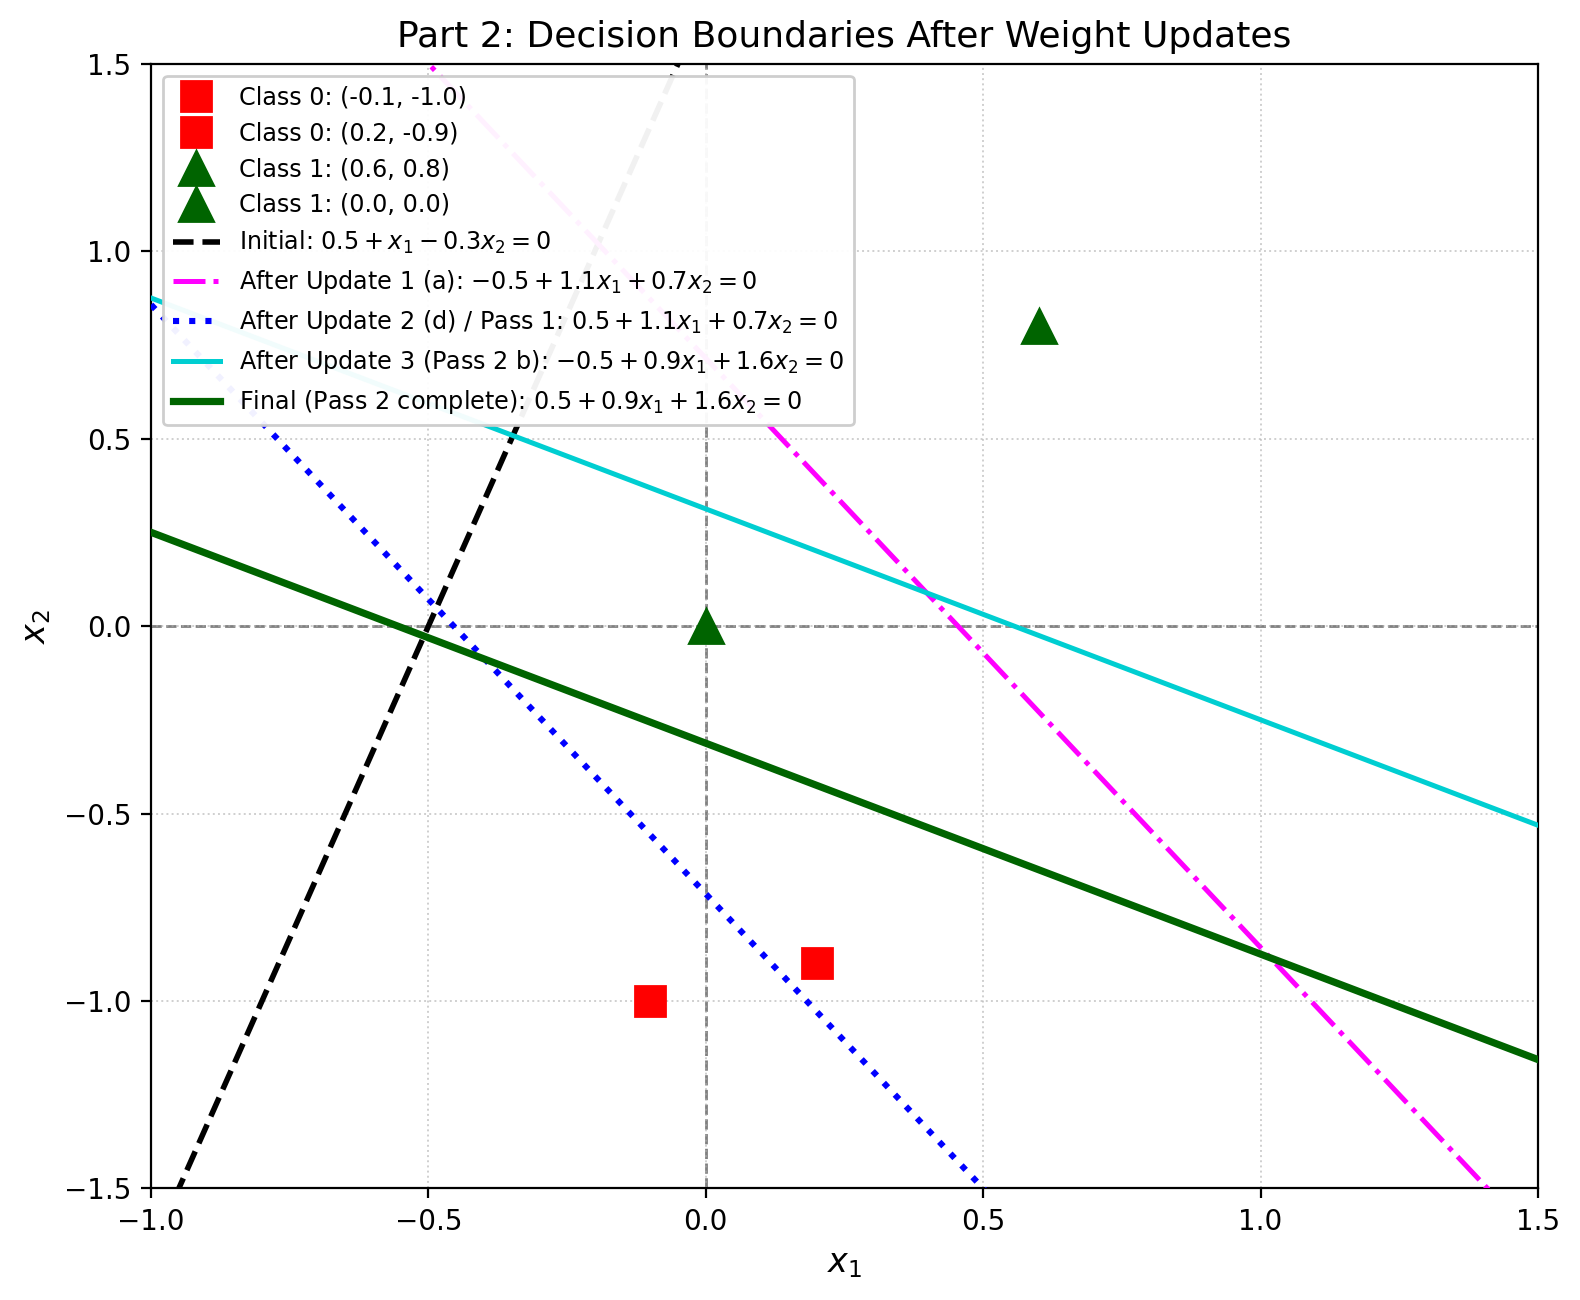
\includegraphics[width=\textwidth]{figures/fig5_part2.png}
\caption{The four training points together with the decision boundary after every weight
update. The black dashed line is the initial boundary, and each subsequent line shows the
boundary immediately after one update. The solid dark green line is the final boundary,
which classifies all four points correctly.}
\end{figure}

\subsection*{2.3\quad Which points are correct after one full pass?}

If we evaluate all four points with the post-pass weights $\bw = (0.5,\,1.1,\,0.7)$:

\begin{table}[H]
\centering
\begin{tabular}{clccccl}
\toprule
& Point & $t$ & $\net = 0.5 + 1.1x_1 + 0.7x_2$ & $a$ & Correct? \\
\midrule
(a) & $(-0.1,\,-1.0)$ & 0 & $0.5 - 0.11 - 0.70 = -0.31$ & 0 & yes \\
(b) & $(0.2,\,-0.9)$  & 0 & $0.5 + 0.22 - 0.63 = +0.09$ & 1 & \textbf{no} \\
(c) & $(0.6,\,0.8)$   & 1 & $0.5 + 0.66 + 0.56 = +1.72$ & 1 & yes \\
(d) & $(0.0,\,0.0)$   & 1 & $0.5 + 0.00 + 0.00 = +0.50$ & 1 & yes \\
\bottomrule
\end{tabular}
\end{table}

\paragraph{Answer.} Points (a), (c) and (d) are correctly classified, while point
\textbf{(b) is misclassified}, at $\net = +0.09$, which is just barely on the wrong side of
the line.

\paragraph{What this tells us about the learning rule.}
Online, or incremental, learning updates the weights instance by instance. Adjusting the
weights in order to correct one sample, such as point (d), can shift the decision boundary
in such a way that a previously correct sample, such as point (b), becomes misclassified.
Thus, a single pass is rarely sufficient, and we need multiple passes, or epochs, in order
to reach full convergence.

\subsection*{2.4\quad How many more passes are needed?}

\paragraph{Answer: \textbf{one} more pass.} After a second pass, all four points are
correctly classified, and a third pass produces no updates at all, which confirms
convergence.

\paragraph{Work for pass 2, starting from $\bw = (0.5,\,1.1,\,0.7)$.}

\begin{align*}
\text{(a) } \bp=(1,-0.1,-1.0),\ t=0:\quad
\net &= 0.5 - 0.11 - 0.70 = -0.31 < 0 \Rightarrow a=0,\quad t-a=0 \ \text{(no change)}\\[4pt]
\text{(b) } \bp=(1,0.2,-0.9),\ t=0:\quad
\net &= 0.5 + 0.22 - 0.63 = +0.09 \ge 0 \Rightarrow a=1,\quad t-a=-1 \\
\bw &\leftarrow (0.5,\,1.1,\,0.7) - (1,\,0.2,\,-0.9) = (-0.5,\;0.9,\;1.6)\\[4pt]
\text{(c) } \bp=(1,0.6,0.8),\ t=1:\quad
\net &= -0.5 + 0.54 + 1.28 = +1.32 \ge 0 \Rightarrow a=1,\quad t-a=0 \ \text{(no change)}\\[4pt]
\text{(d) } \bp=(1,0,0),\ t=1:\quad
\net &= -0.5 < 0 \Rightarrow a=0,\quad t-a=+1 \\
\bw &\leftarrow (-0.5,\,0.9,\,1.6) + (1,\,0,\,0) = \mathbf{(0.5,\;0.9,\;1.6)}
\end{align*}

\paragraph{Check of all four points with $\bw = (0.5,\,0.9,\,1.6)$:}

\begin{table}[H]
\centering
\begin{tabular}{clcccl}
\toprule
& Point & $t$ & $\net = 0.5 + 0.9x_1 + 1.6x_2$ & $a$ & Correct? \\
\midrule
(a) & $(-0.1,\,-1.0)$ & 0 & $0.5 - 0.09 - 1.60 = -1.19$ & 0 & yes \\
(b) & $(0.2,\,-0.9)$  & 0 & $0.5 + 0.18 - 1.44 = -0.76$ & 0 & yes \\
(c) & $(0.6,\,0.8)$   & 1 & $0.5 + 0.54 + 1.28 = +2.32$ & 1 & yes \\
(d) & $(0.0,\,0.0)$   & 1 & $0.5 + 0.00 + 0.00 = +0.50$ & 1 & yes \\
\bottomrule
\end{tabular}
\end{table}

All four of them are correct, so pass 3 encounters $t - a = 0$ at every point and leaves
$\bw = (0.5,\,0.9,\,1.6)$ unchanged. The algorithm has converged. On the scale suggested in
the question, the answer is \textbf{one}.

\subsection*{2.5\quad Effect of introducing a learning rate $\eta$}

If we introduce a learning rate $\eta \in (0, 1]$, the update rule becomes
\[
\bw_{\text{new}} \;=\; \bw_{\text{old}} + \eta\,(t - a)\,\bp .
\]

\begin{enumerate}[leftmargin=1.6em,itemsep=3pt]
\item \textbf{Controlled step size.} Scaling the updates by $\eta$ moderates the magnitude
of the weight adjustment that we need to make at each step.
\item \textbf{Improved stability.} Smaller updates prevent wild oscillations of the
boundary, which keeps previously correctly classified points stable.
\item \textbf{Convergence rate.} While small learning rates ensure smoother convergence,
they may increase the total number of passes that we have to perform in order to achieve
full separation.
\end{enumerate}

\clearpage
\noindent\rule{\textwidth}{0.4pt}

\section*{Appendix: Handwritten Work}

\begin{figure}[H]
\centering
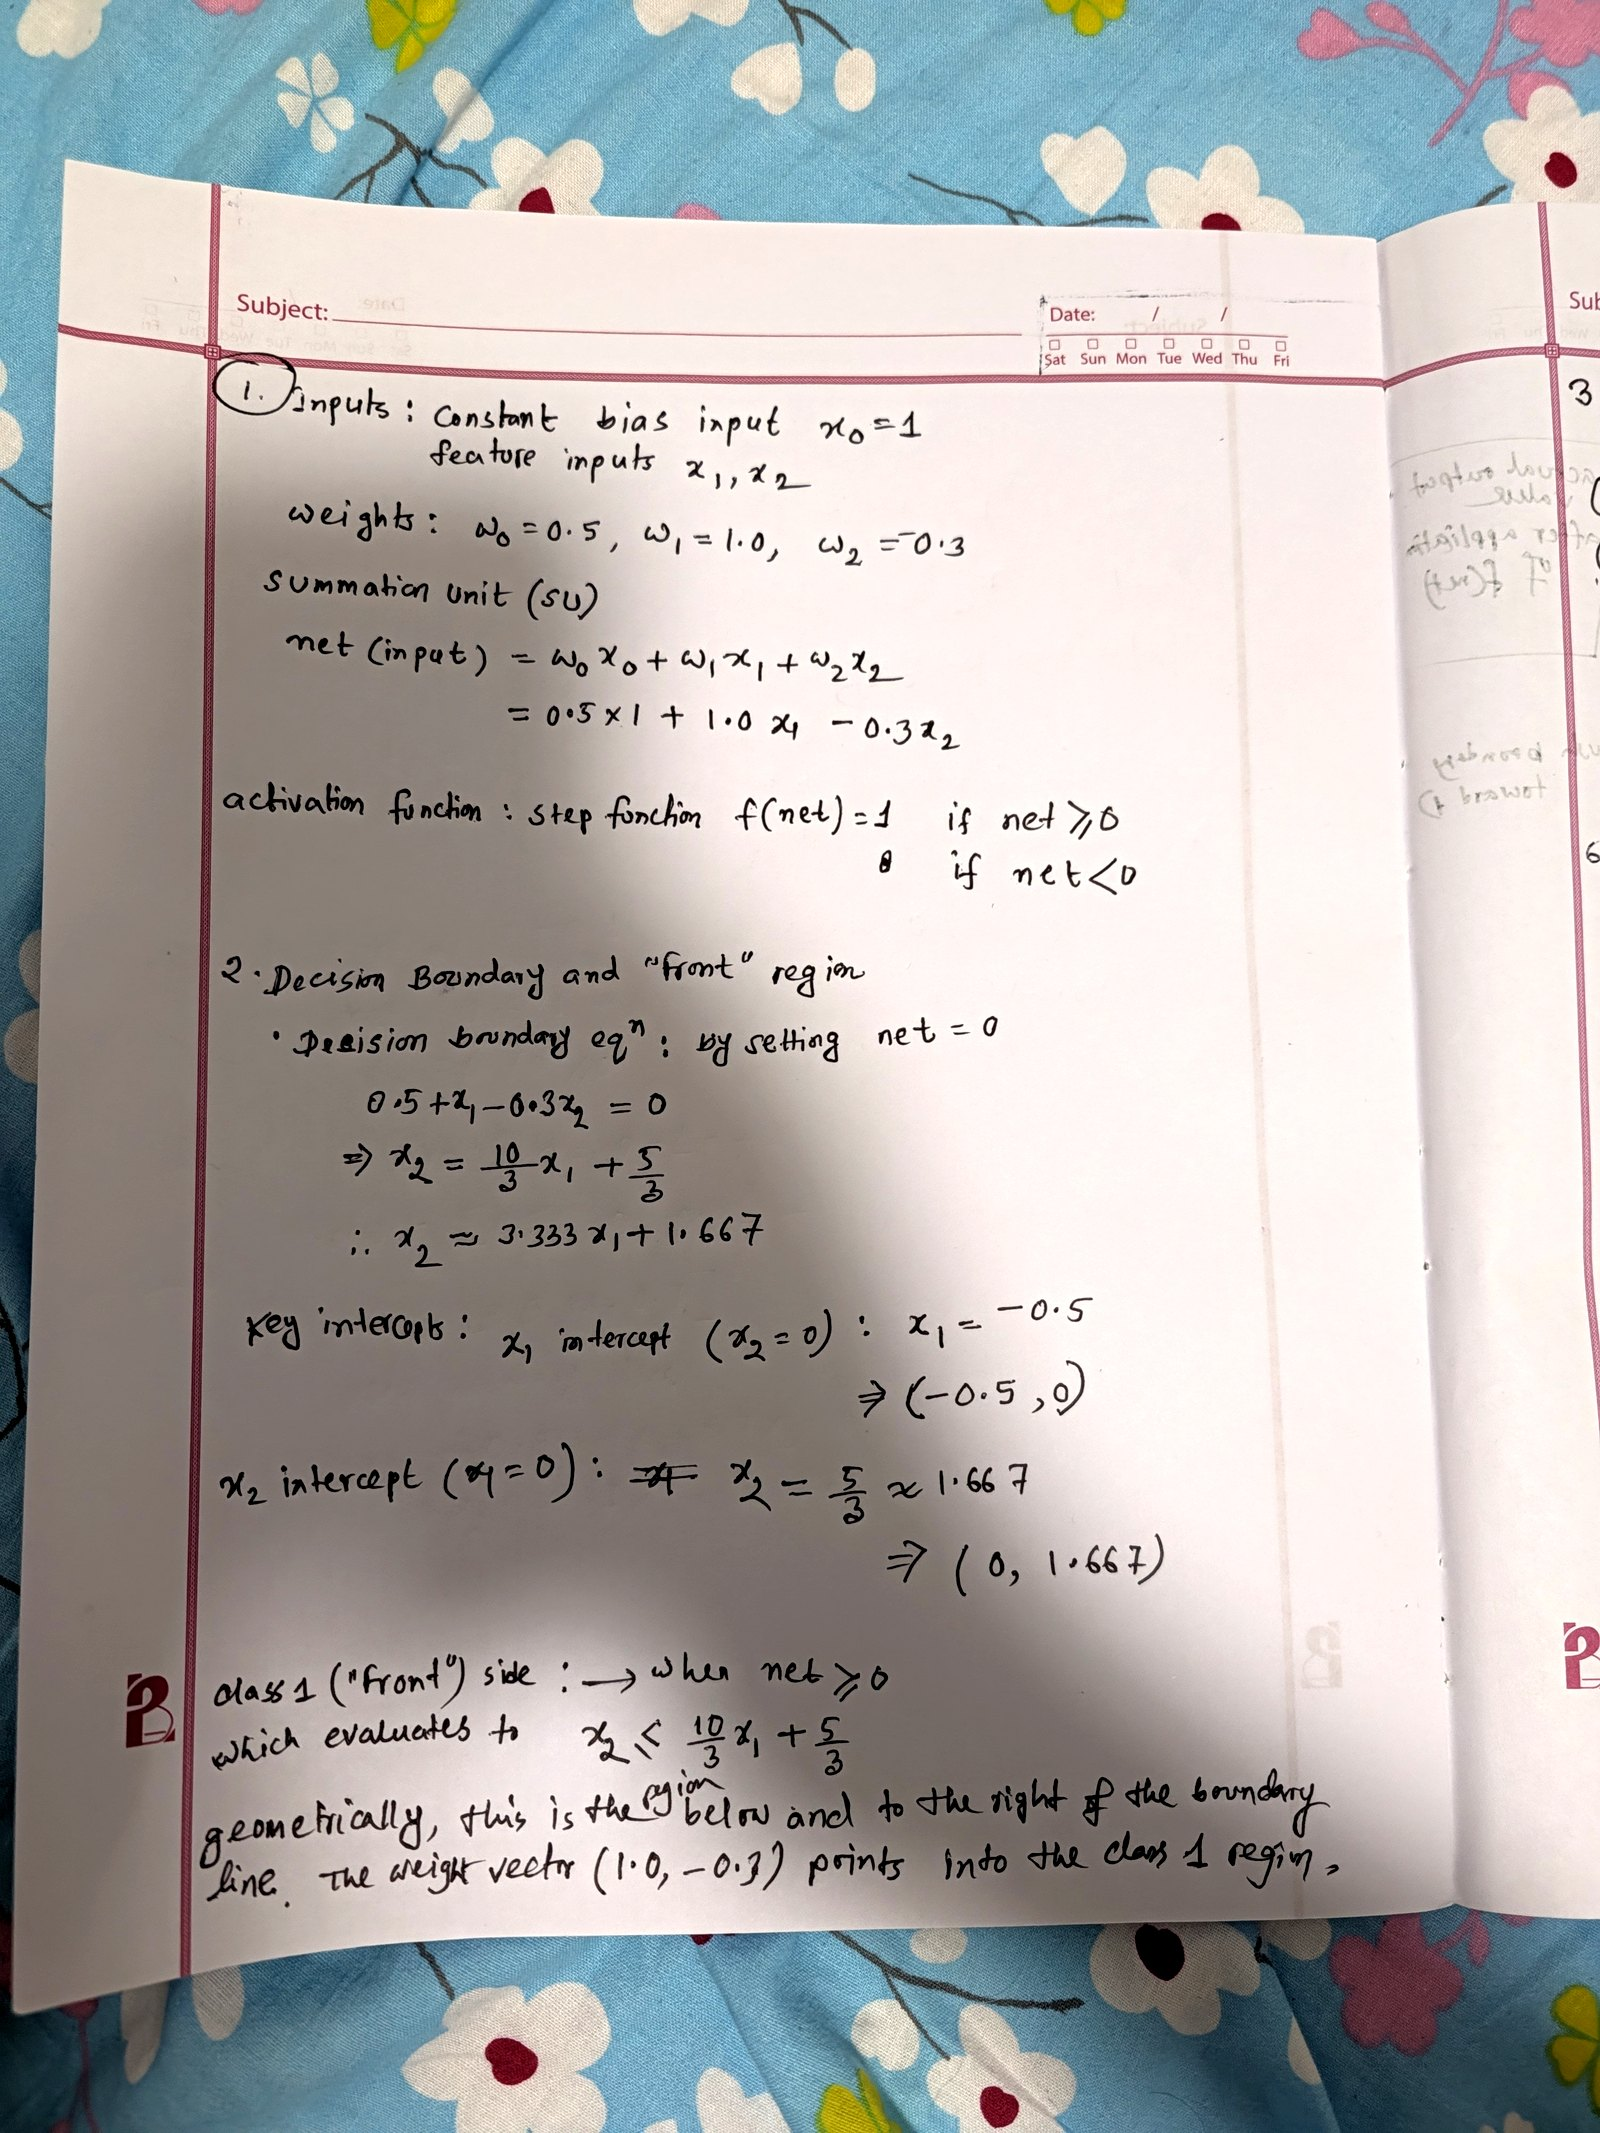
\includegraphics[width=0.86\textwidth]{handwritten/hw_p1.jpg}
\caption{Handwritten work, page 1: questions 1.1 and 1.2.}
\end{figure}

\clearpage
\begin{figure}[H]
\centering
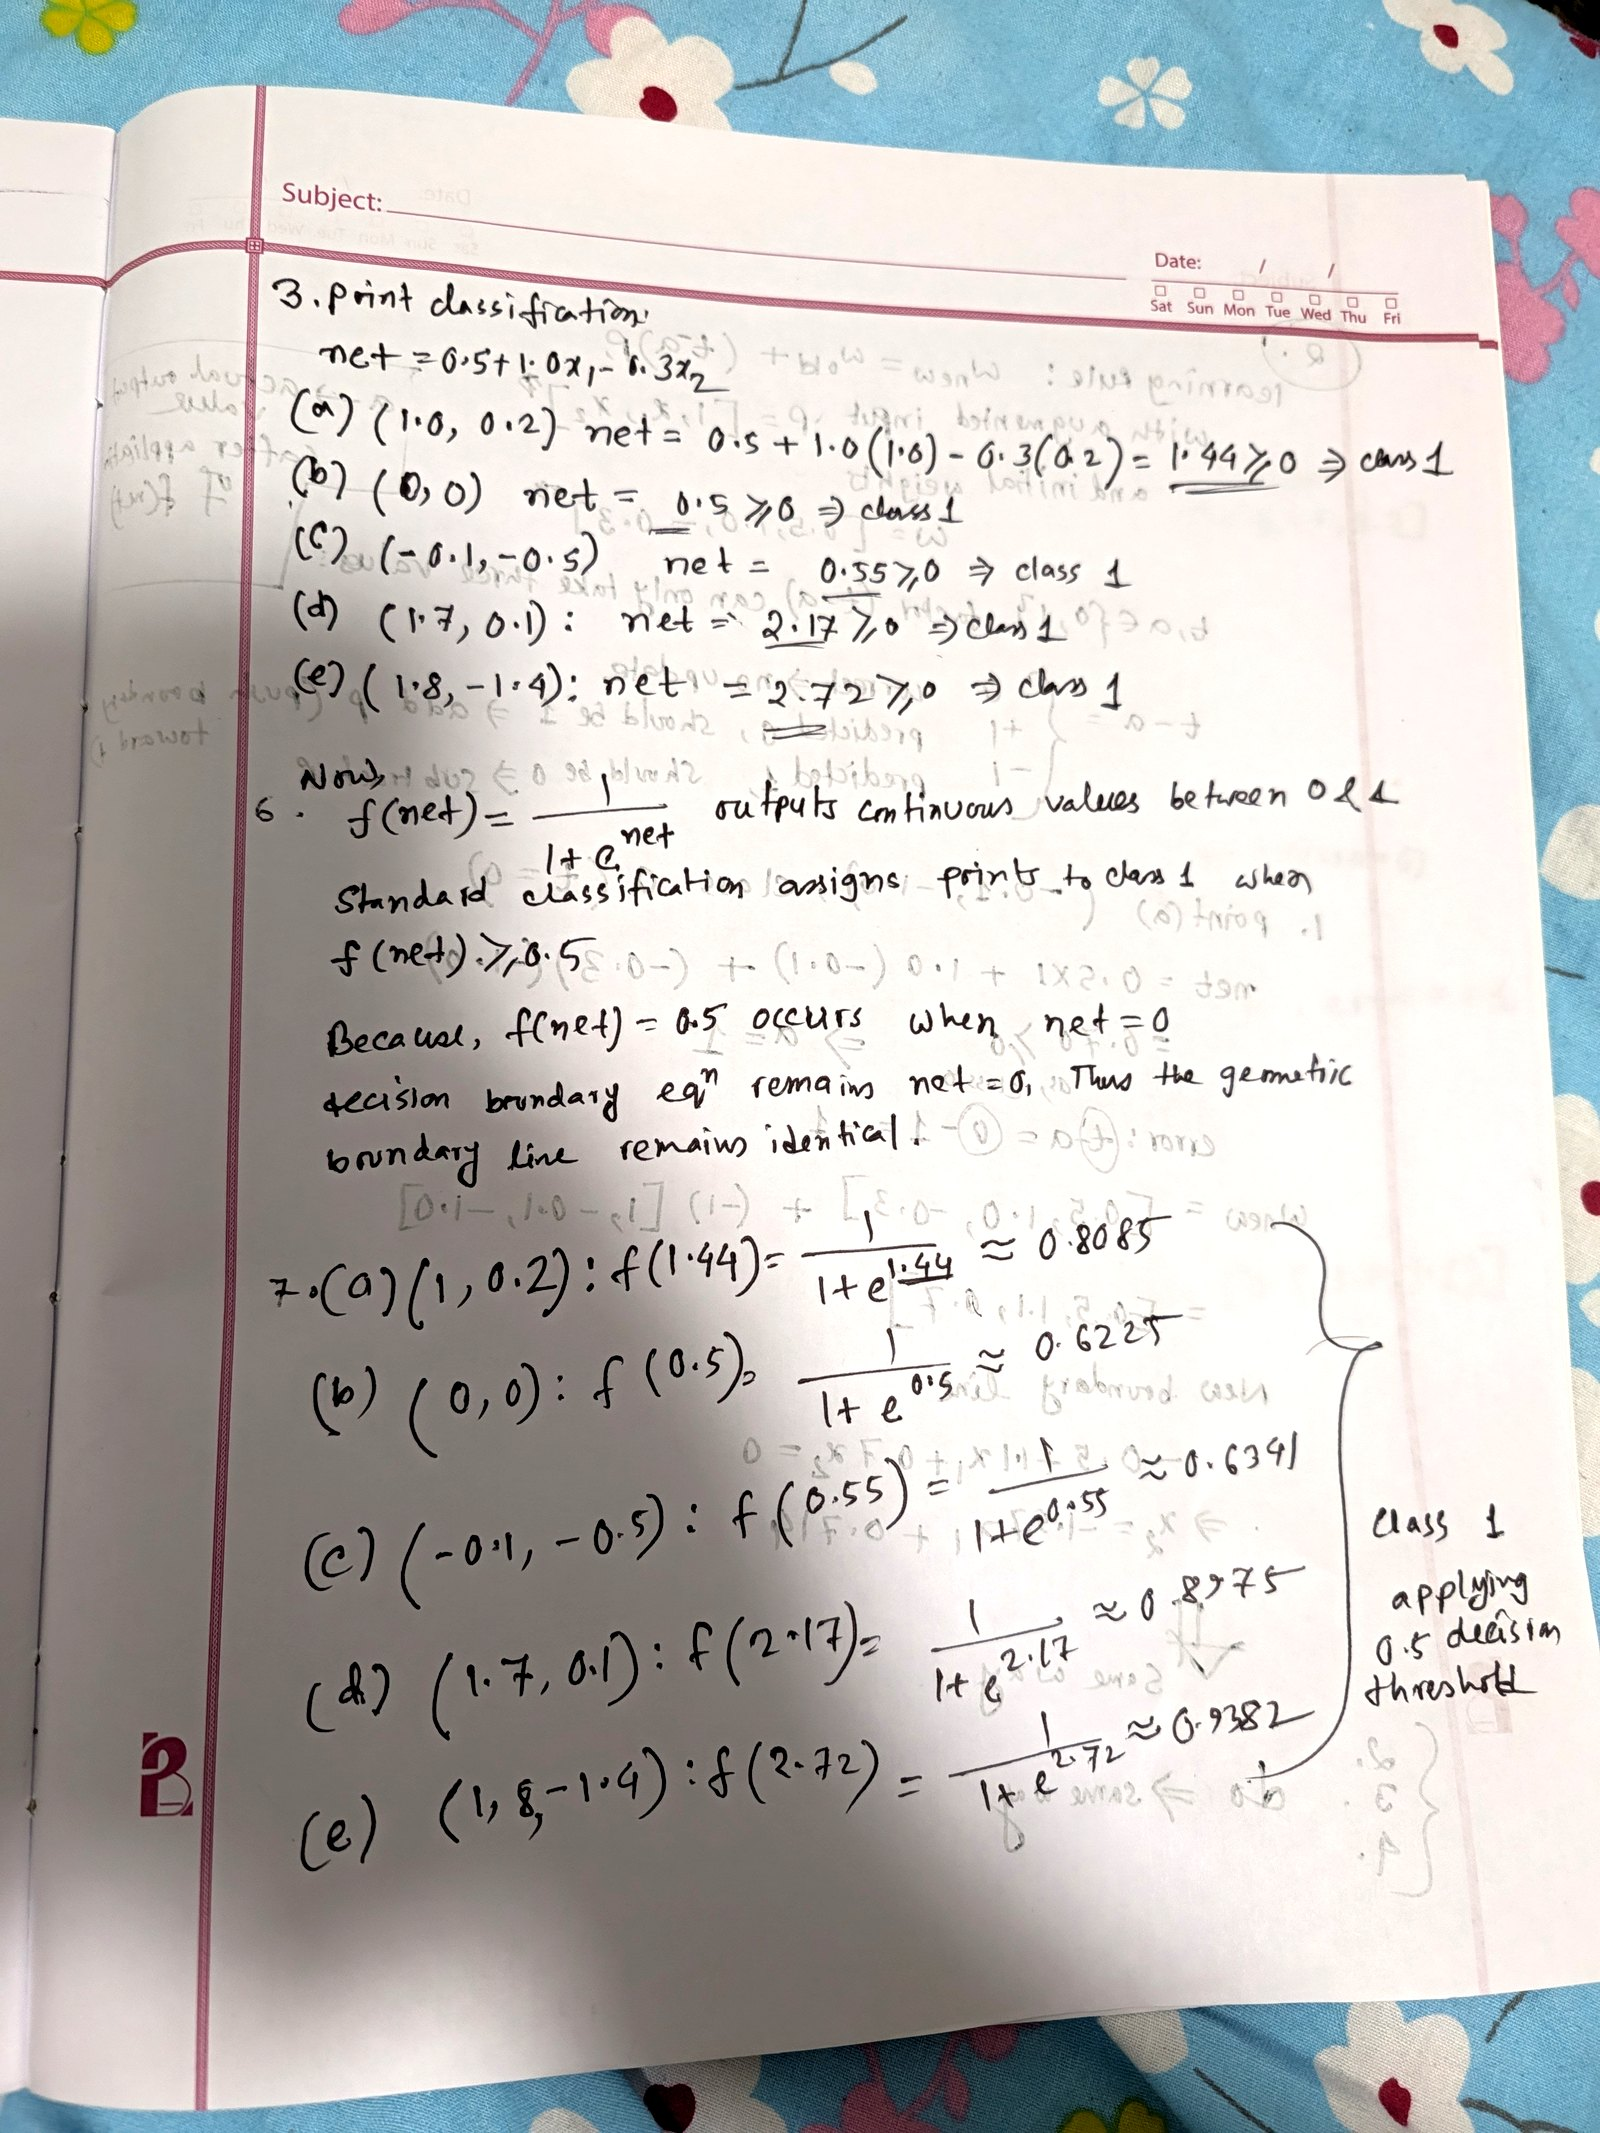
\includegraphics[width=0.86\textwidth]{handwritten/hw_p2.jpg}
\caption{Handwritten work, page 2: questions 1.3, 1.6 and 1.7.}
\end{figure}

\clearpage
\begin{figure}[H]
\centering
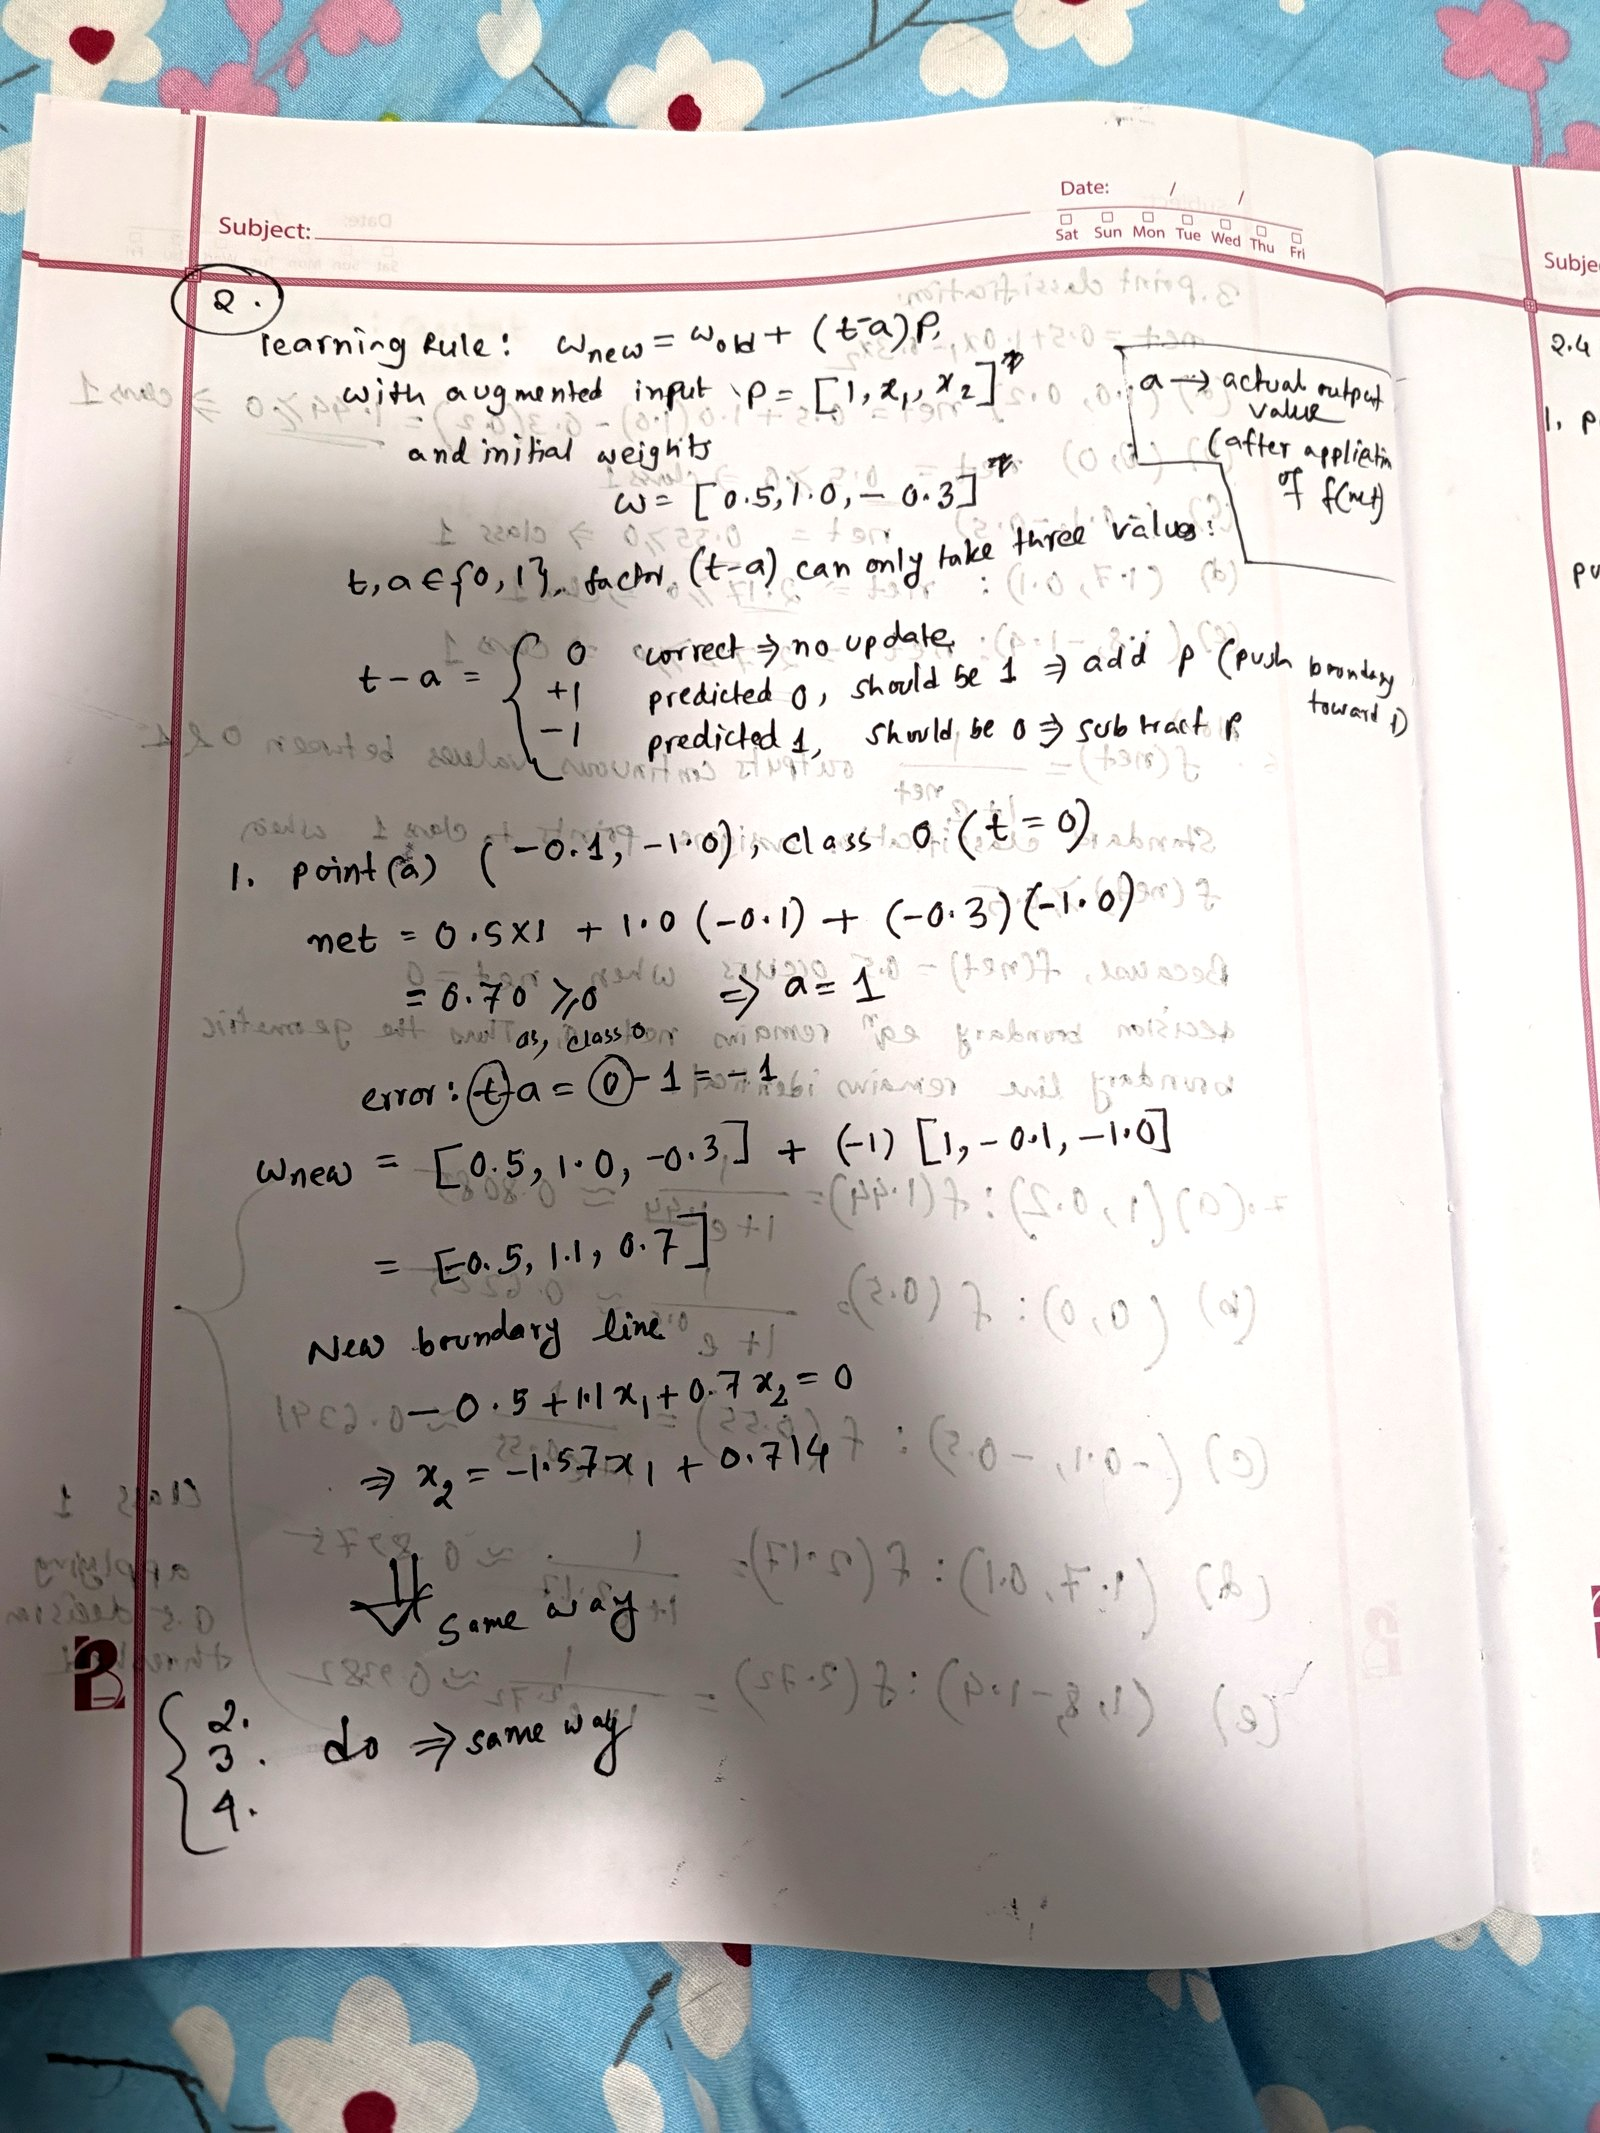
\includegraphics[width=0.86\textwidth]{handwritten/hw_p3.jpg}
\caption{Handwritten work, page 3: question 2.1, the learning rule and the update at
point (a).}
\end{figure}

\clearpage
\begin{figure}[H]
\centering
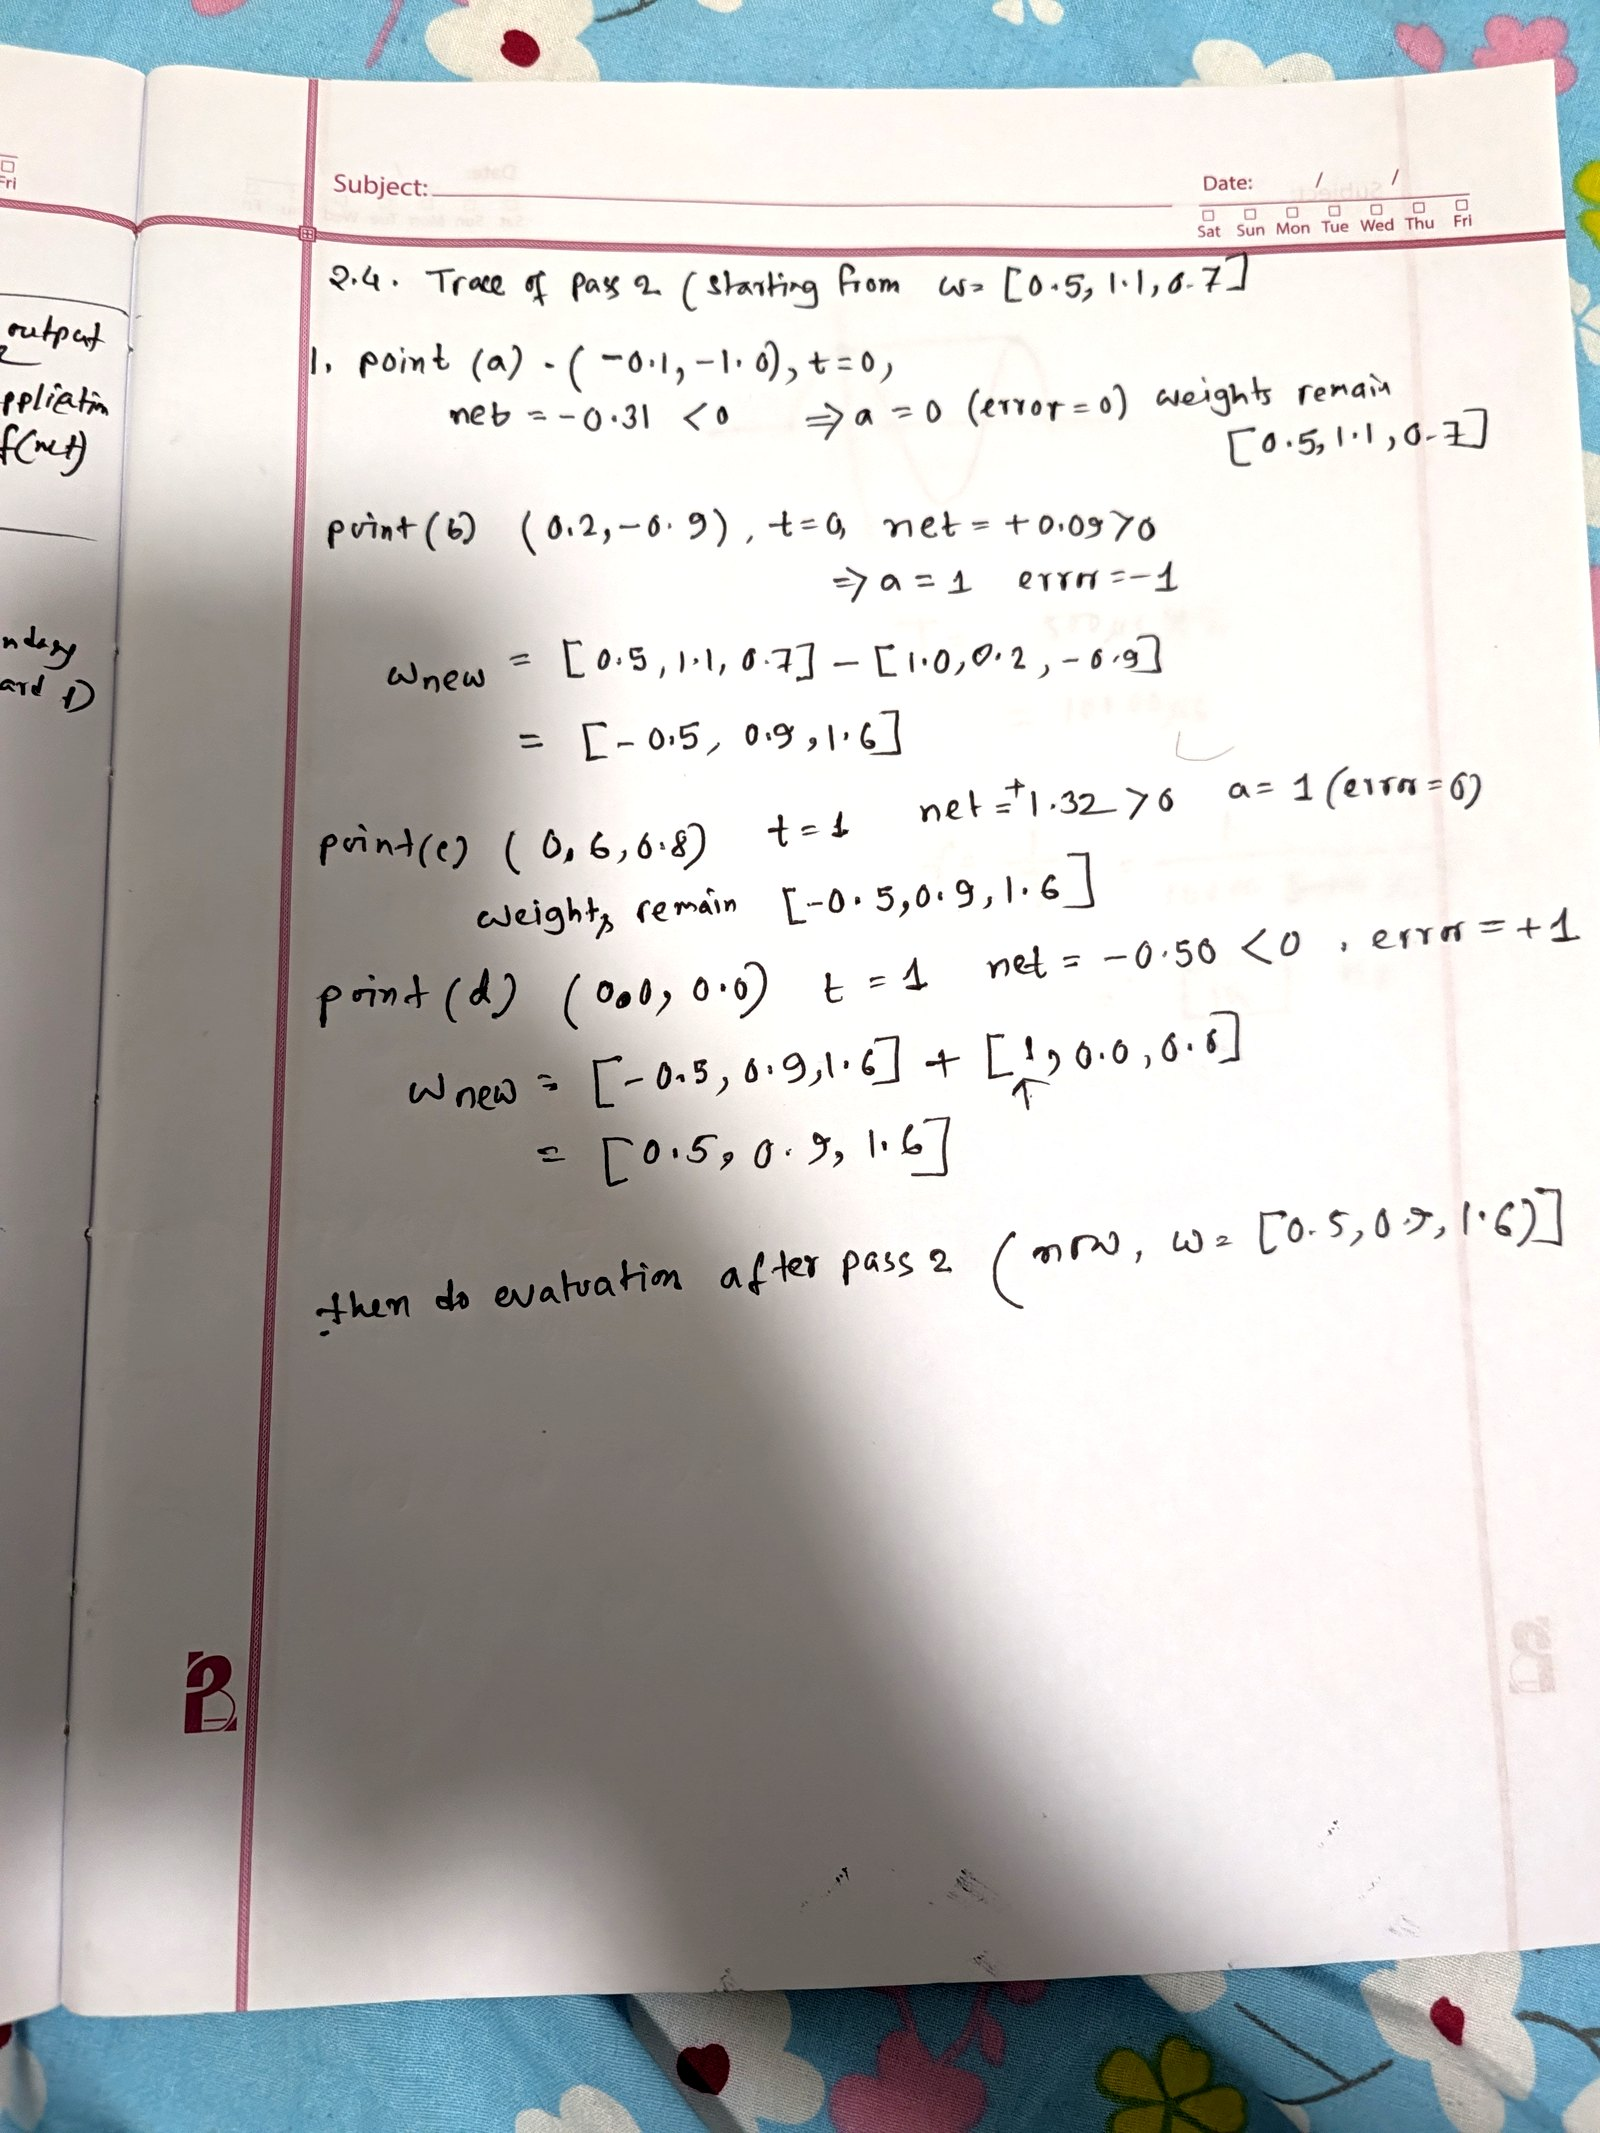
\includegraphics[width=0.86\textwidth]{handwritten/hw_p4.jpg}
\caption{Handwritten work, page 4: question 2.4, the trace of pass 2.}
\end{figure}

\vfill
\noindent\rule{\textwidth}{0.4pt}
{\footnotesize \textit{AI use disclosure: an AI assistant (Claude) was used while working
through this assignment.}}

\end{document}
